\section{Updated Opacities}\label{sec:opac}
% Radiative opacity is fundamental to stellar structure, it determines how much
% incident radiation is absorbed or scattered. Moreover, when a media is in
% thermodynamic equilibrium with the radiation field, that is when the temperature
% of the media and that of the radiation field is the same, the opacity may be
% used via Kirchhoff's law to find the emissivity of a material
% \citep{Huebner2014}. Local Thermodynamic Equilibrium (LTE) is a common state to
% find within a star and therefore stellar models have long relied on opacities
% calculated in LTE.
Multiple groups have released high-temperature opacities including, the Opacity
Project \citep[OP][]{Seaton1994}, Laurence Livermore National Labs OPAL opacity
tables \citep{Iglesias1996}, and Los Alamos National Labs OPLIB opacity tables
\citep{Colgan2016}. OPAL high-temperature radiative opacity tables in
particular are very widely used by current generation isochrone grids
\citep[e.g. Dartmouth, MIST, \& StarEvol, ][]{Dotter2008,Choi2016,Amard2019}.
OPLIB opacity tables \citep{Colgan2016} are not widely used but include the
most up-to-date plasma modeling.

While the overall effect on the CMD of using OPLIB compared to OPAL tables is
small, the strong theoretical opacity dependence of the Jao Gap raises the
potential for these small effects to measurably shift the Gap's location. We
update DSEP to use high temperature opacity tables based on measurements from
Los Alamos national Labs T-1 group \citep[OPLIB,][]{Colgan2016}. The OPLIB
tables are created with ATOMIC \citep{Magee2004,Hakel2006,Fontes2016}, a modern
LTE and non-LTE opacity and plasma modeling code. These updated tables were
initially created in order to incorporate the most up to date plasma
physics at the time \citep{Bahcall2005}. 

OPLIB tables include monochromatic Rosseland mean opacities --- composed from
bound-bound, bound-free, free-free, and scattering opacities --- for elements
hydrogen through zinc over temperatures 0.5eV to 100 keV (5802 K -- 1.16$\times
10 ^{9}$ K) and for mass densities from approximately $10^{-8}$ g cm$^{-3}$ up
to approximately $10^{4}$ g cm$^{-3}$ (though the exact mass density range
varies as a function of temperature). 

DSEP ramps the \citet{Ferguson2005} low temperature opacities to high
temperature opacities tables between $10^{4.3}$ K and $10^{4.5}$ K; therefore,
only differences between high-temperature opacity sources above $10^{4.3}$ K
can effect model evolution. When comparing OPAL and OPLIB opacity tables
(Figure \ref{fig:opacComp}) we find OPLIB opacities are systematically lower
than OPAL opacities for temperatures above $10^{5}$ K. Between $10^{4.3}$ and
$10^{5} K$ OPLIB opacities are larger than OPAL opacities. These generally
lower opacities will decrease the radiative temperature gradient throughout
much of the radius of a model.

\begin{figure}
	\centering
	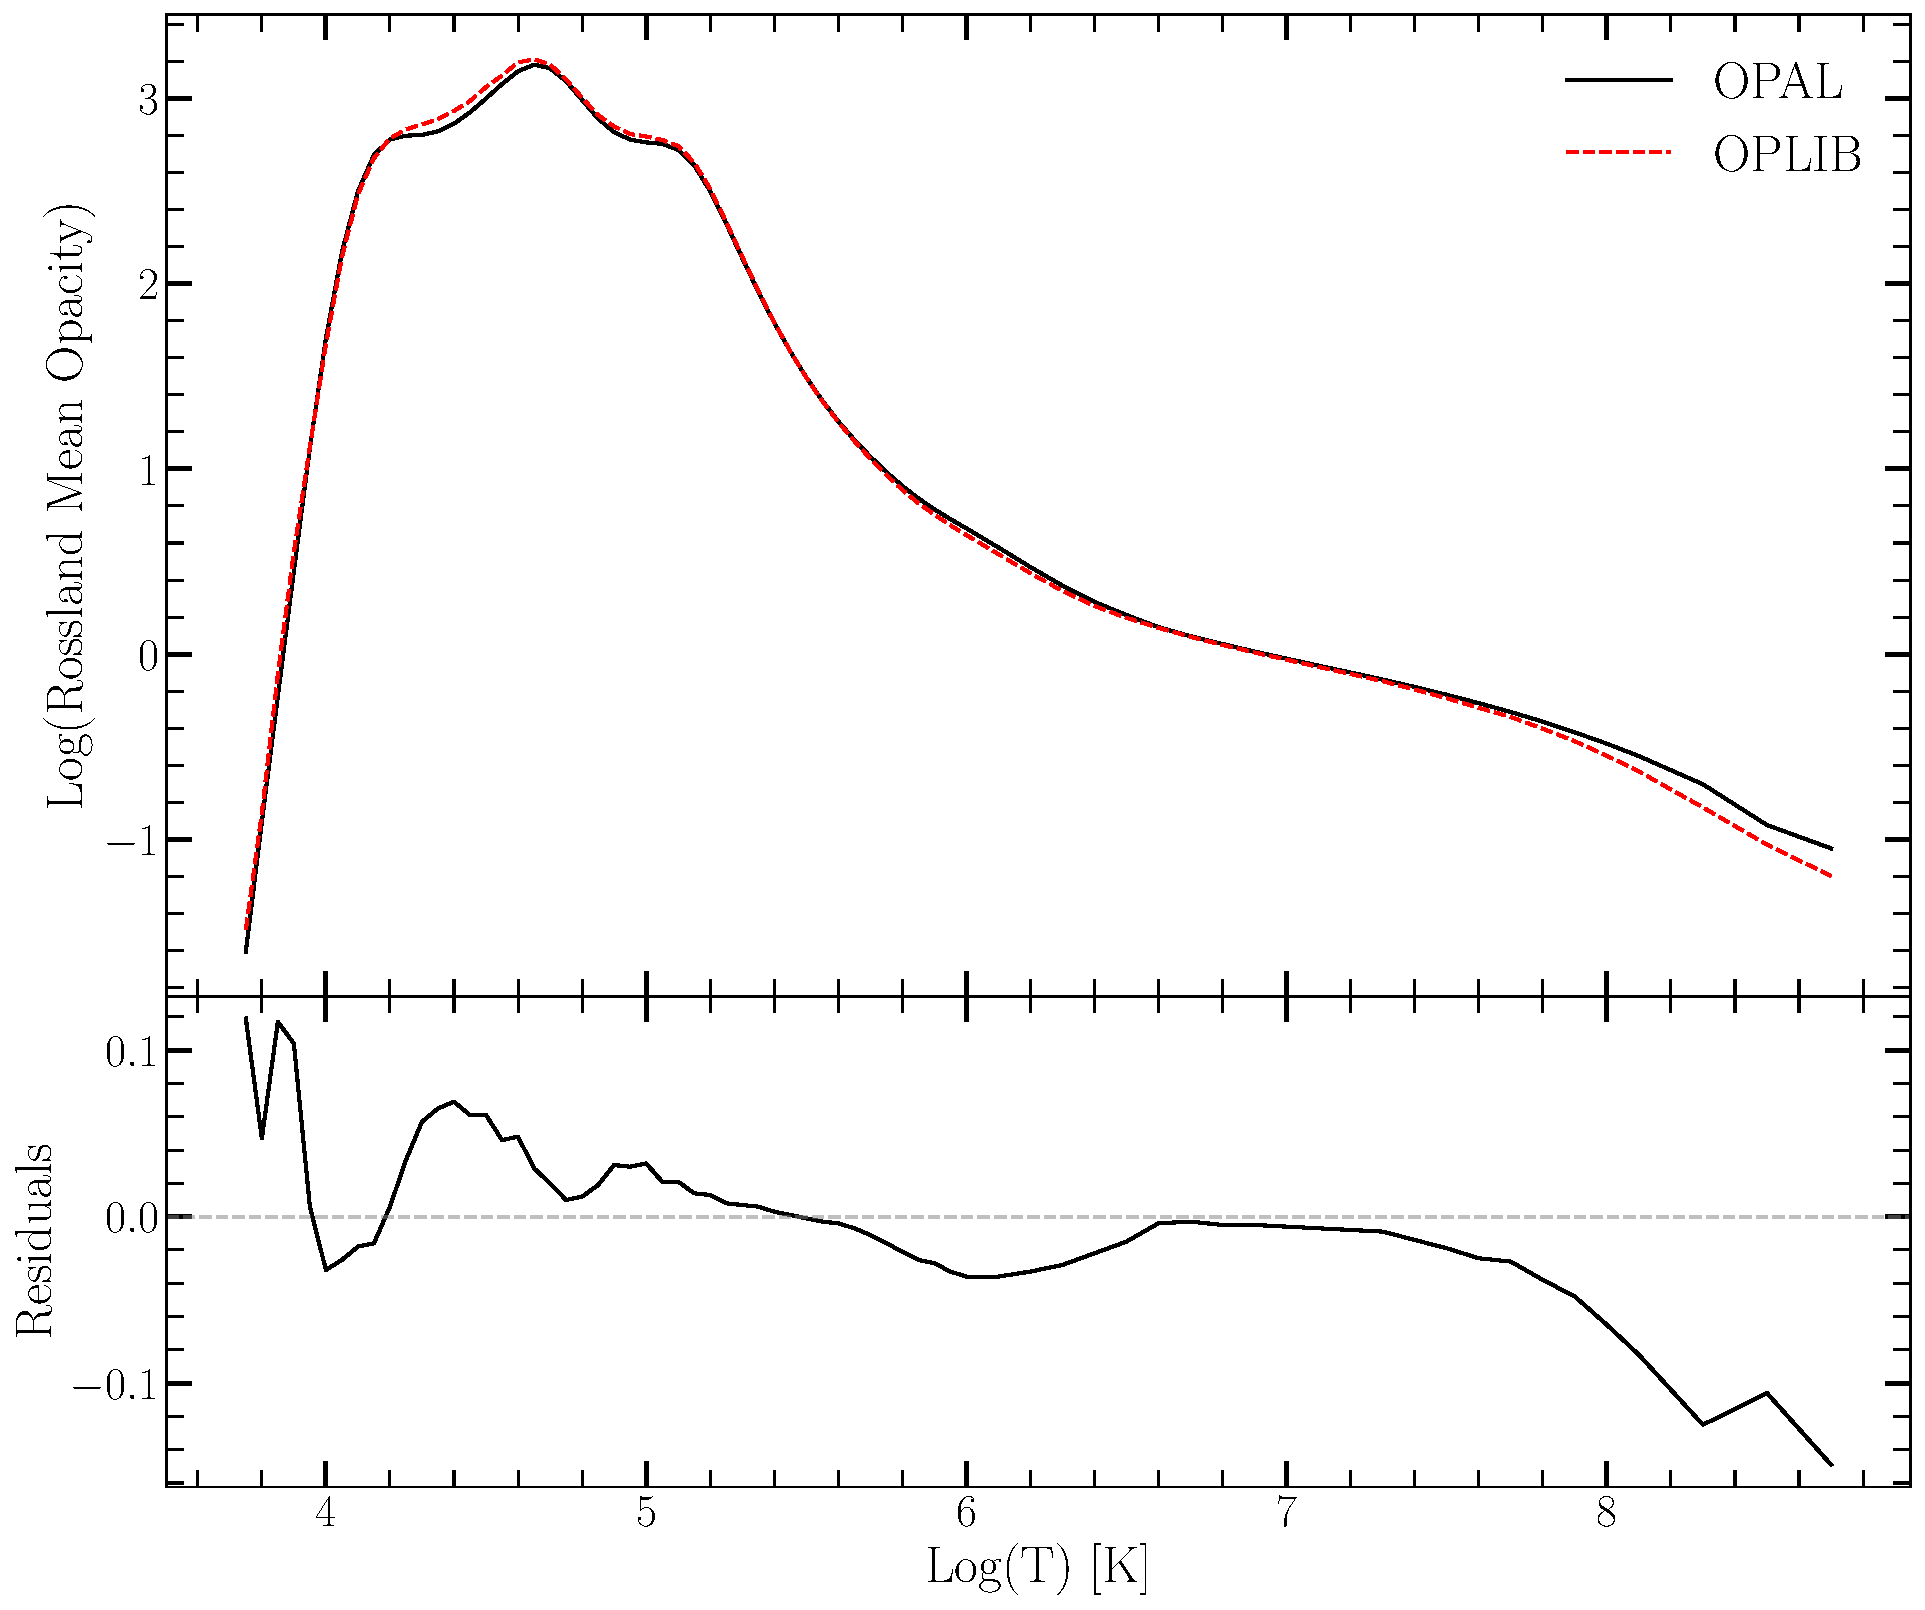
\includegraphics[width=0.45\textwidth]{OpacityComparision.pdf}
	\caption{Rosseland mean opacity with the GS98 solar composition for both
	OPAL opacities and OPLIB opacities (top). Residuals between OPLIB opacities
	and OPAL opacities (bottom). These opacities are plotted at $\log _{10}(R)
	= -0.5$, $X=0.7$, and $Z=0.02$. $\log _{10}(R)=-0.5$ approximates
	much of the interior a 0.35 M$_{\odot}$ model. Note how the OPLIB
	opacities are systematically lower than the OPAL opacities for temperatures
	above $10^{5.2}$ K.}
	\label{fig:opacComp}
\end{figure}

\subsection{Table Querying and Conversion}
The high-temperature opacity tables used by DSEP and most other stellar
evolution programs give Rosseland-mean opacity, $\kappa_{R}$, along three
dimensions: temperature, a density proxy $R$ (Equation \ref{eqn:R}; $T_{6} =
T\times10^{-6}$, $\rho$ is the mass density), and composition. 

\begin{align} \label{eqn:R}
	R = \frac{\rho}{T_{6}^{3}}
\end{align}

OPLIB tables may be queried from a web
interface\footnote{https://aphysics2.lanl.gov/apps/}; however, OPLIB opacities
are parametrized using mass-density and temperature instead of $R$ and
temperature. It is most efficient for us to convert these tables to the OPAL
format instead of modifying DSEP to use the OPLIB format directly. In order to
generate many tables easily and quickly we develop a web scraper
\citep[\texttt{pyTOPSScrape},][]{Boudreaux22} which can automatically retrieve
all the tables needed to build an opacity table in the OPAL format.
\texttt{pyTOPSScrape}\footnote{https://github.com/tboudreaux/pytopsscrape} has
been released under the permissive \texttt{MIT} license with the consent of the
Los Alamos T-1 group. For a detailed discussion of how the web scraper works
and how OPLIB tables are transformed into a format DSEP can use see Appendices
\ref{apx:pytopsscrape} \& \ref{apx:interp}.

\subsection{Solar Calibrated Stellar Models}\label{sec:SCSM}
% In order to further validate the OPLIB high-temperature opacities we first visually
% compare a set of opacity vs. temperature curves from OPLIB at a constant $R$
% and \citet{Grevesse1998} composition (GS98) to the same curve from OPAL. A
% characteristic opacity vs temperature curve is shown in Figure
% \ref{fig:OpacCompare}, $\log _{10}(R) = -1.5$ is chosen as for much of the
% radius of a main sequence star $\log _{10}(R)$ is around that value. The
% largest variation in $\kappa_{R}$ from OPAL to OPLIB at $\log _{10}(R)=-1.5$ is
% on the order of a few percent. This is inline with expectations of OPLIB and OPAL
% being in relatively close agreement \citep{Colgan2016}.


In order to validate the OPLIB opacities, we generate a solar calibrated
stellar model (SCSM) using these new tables. We first manually calibrate the
surface Z/X abundance to within one part in 100 of the solar value \citep[][Z/X=0.23]{Grevesse1998}.
Subsequently, we allow both the convective mixing length parameter,
$\alpha_{ML}$, and the initial Hydrogen mass fraction, $X$, to vary
simultaneously, minimizing the difference, to within one part in $10^{5}$,
between resultant models' final radius and luminosity to those of the sun.
Finally, we confirm that the model's surface Z/X abundance is still within one
part in 100 of the solar value.

\begin{figure}
	\centering
	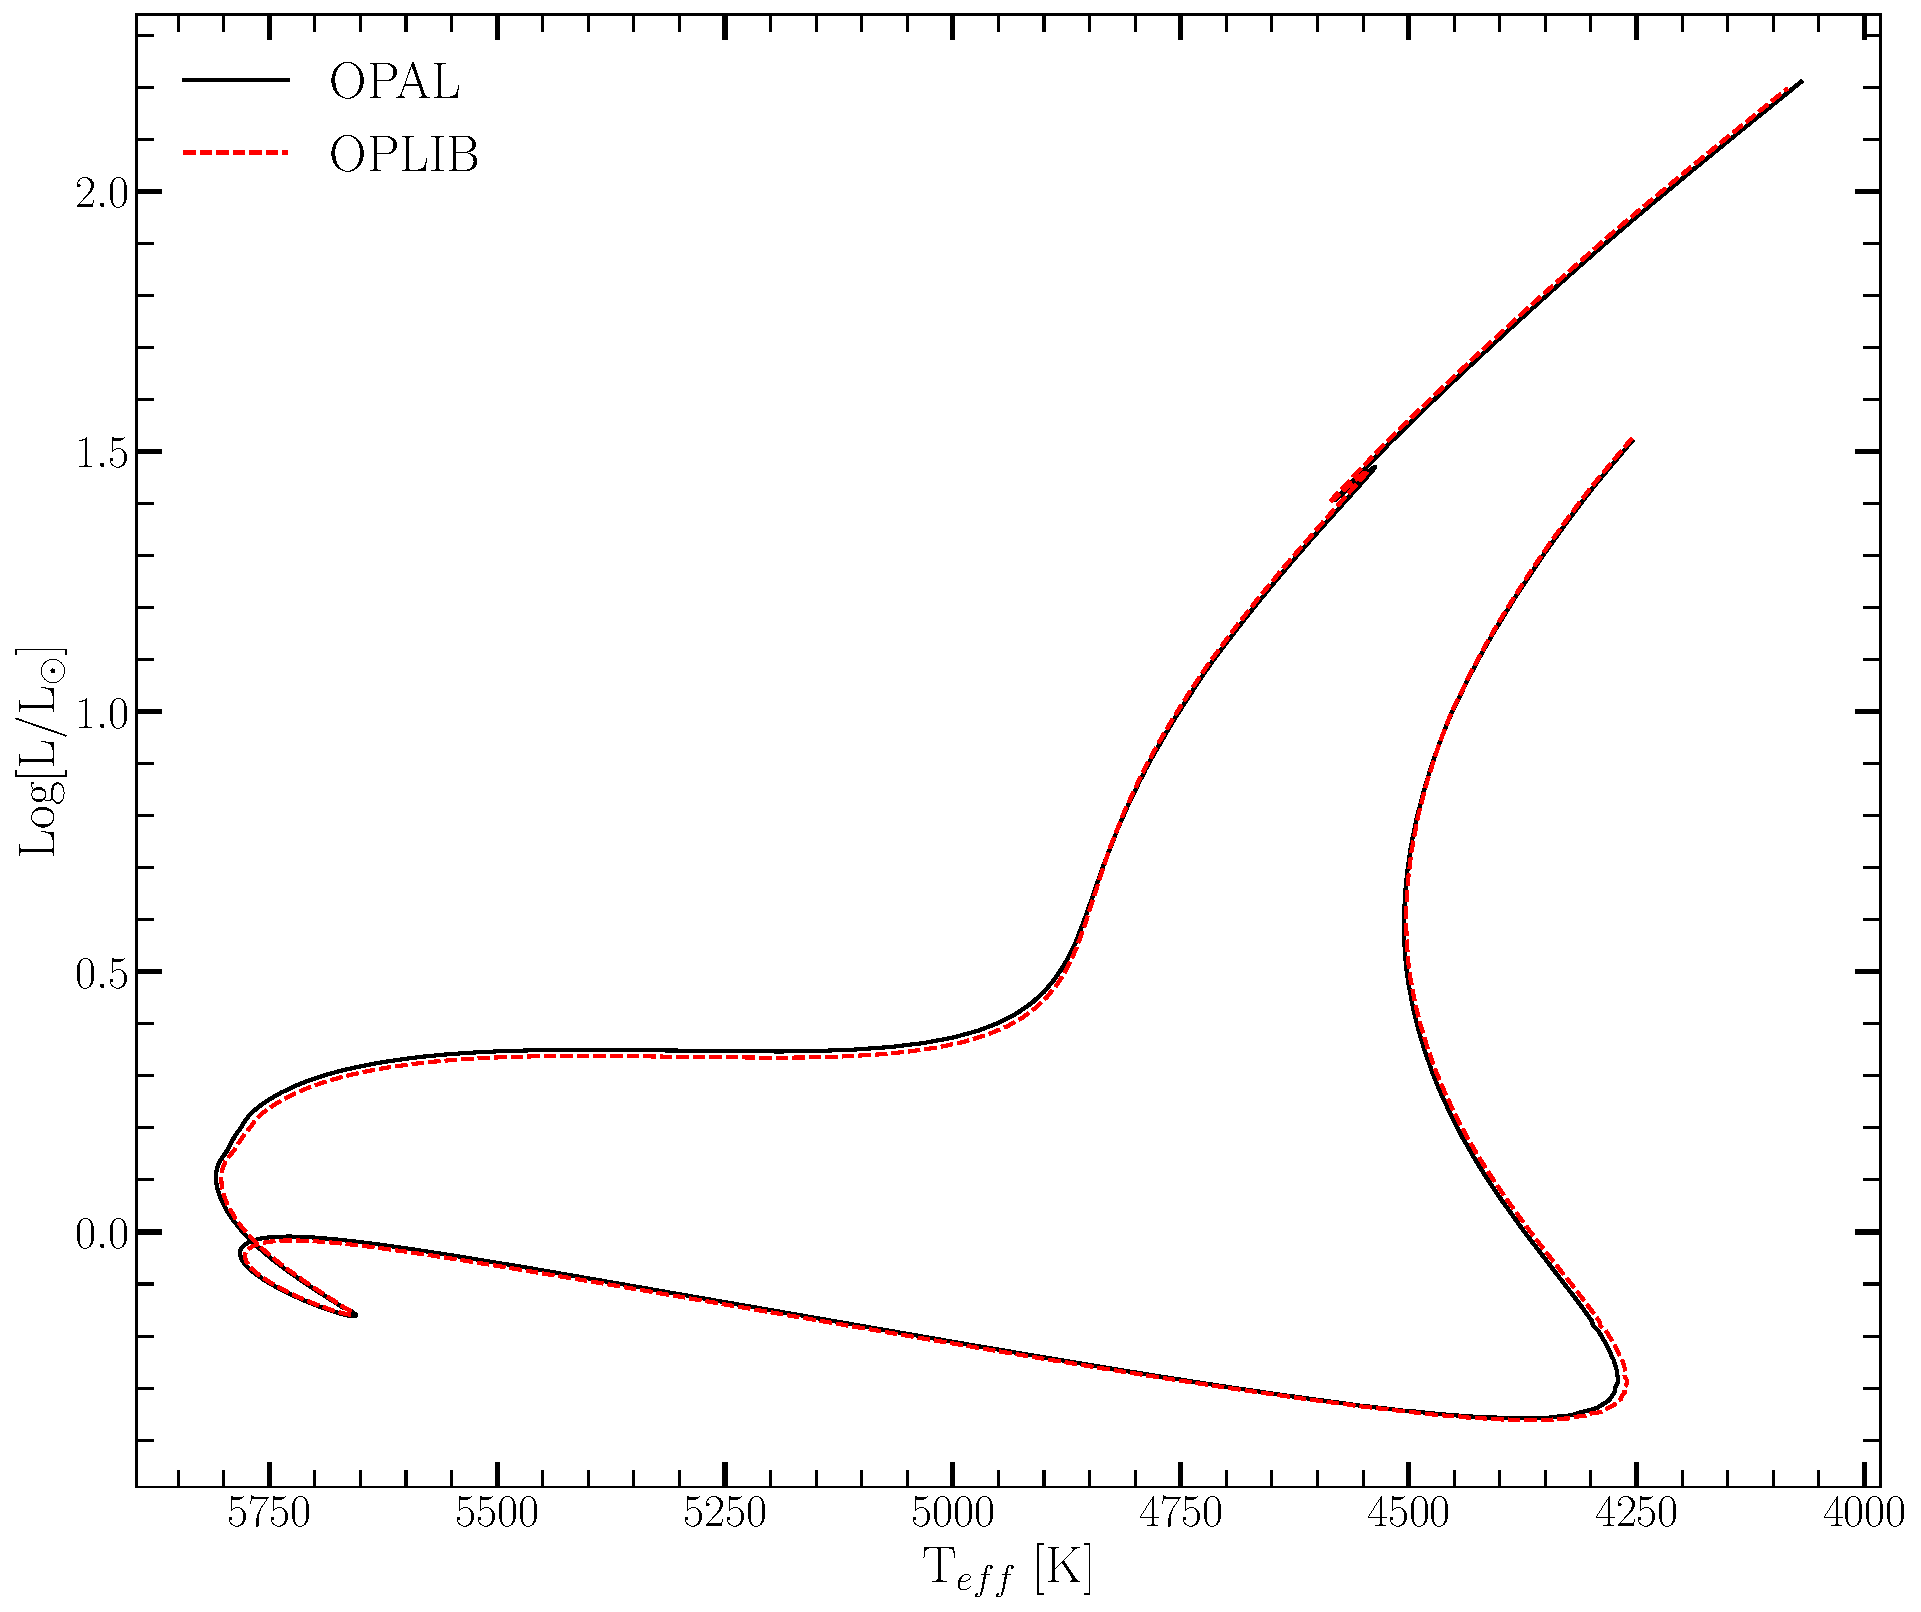
\includegraphics[width=0.45\textwidth]{HRDiagramOPALvsOPLIB_SCCM.pdf}
	\caption{HR Diagram for the two SCSMs, OPAL and OPLIB. OPLIB is shown as a red
	dashed line.}
	\label{fig:OPLIBOPALHR}
\end{figure}

Solar calibrated stellar models evolved using GS98 OPAL and OPLIB opacity
tables (Figure \ref{fig:OPLIBOPALHR}) differ $\sim 0.5\%$ in the SCSM hydrogen
mass fractions and $\sim 1.5\%$ in the SCSM convective mixing length parameters
(Table \ref{tab:SCSMResults}). While the two evolutionary tracks are very
similar, note that the OPLIB SCSM's luminosity is systematically lower past the
solar age. While at the solar age the OPLIB SCSM luminosity is effectively the
same as the OPAL SCSM. This luminosity difference between OPAL and OPLIB based
models is not inconsistent with expectations given the more shallow radiative
temperature gradient resulting from the lower OPLIB opacities

\begin{table}
	\centering
	\begin{tabular}{l c c}
		\hline
		Model & $X$ & $\alpha_{ML}$ \\
		\hline
		\hline
		OPAL & 0.7066 & 1.9333 \\
		OPLIB & 0.7107 & 1.9629
	\end{tabular}
	\caption{Optimized parameters for SCSMs evolved using OPAL and OPLIB high
	temperature opacity tables.}
	\label{tab:SCSMResults}
\end{table}

